%% Default Latex document template
%%
%%  blake@rcs.ee.washington.edu

\documentclass[letterpaper]{article}

% Uncomment for bibliog.
\bibliographystyle{unsrt}

\usepackage{graphicx}
\usepackage{lineno}
\usepackage{amsmath}

%\usepackage{fancyhdr}

%%%%%%%%%%%%%%%%%%%%%%%%%%%%%%%%%%%%%%%%5
%
%  Set Up Margins

%%%%%%%%%%%%%%%%%%%%%%%%%%%%%%%%%%%%%%%%%%%%%%%%%
% include file for:
%      Critical Page setup dimensions
%            DO NOT MODIFY
%       (for help see "Latex Line by Line" p 260)
%
\setlength\oddsidemargin{0in}
\setlength\evensidemargin{0in}

\usepackage[left=0.98in, right=0.98in, top=1.0in, bottom=1.0in]{geometry}

% %Top Margin and header
% \setlength\voffset{-0.94in}
% \setlength\topmargin{0.25in}
% \setlength\headheight{0.25in}
% %\setlength\headwidth{6.5in}
% \setlength\headsep{0.25in}
% %Body
% \setlength\textwidth{6.5in}
% \setlength\textheight{9.50in}
% %Footer
% %\setlength\footheight{0.5in}
% \setlength\footskip{0.3750in}
% Line spacing for 6 lines per inch
\linespread{0.894}  % 1.0 = single    1.6 = double
%
%          END of Critical Page Setup Dimensions
%%%%%%%%%%%%%%%%%%%%%%%%%%%%%%%%%%%%%%%%%%%%%%%%%%%

%%%%%%%%%%%%%%%%%%%%%%%%%%%%%%%%%%%%%%%%%%%%%%%%%%%
%
% Useful style and math macros
%


\newcommand\Dfrac[2]{\frac{\displaystyle #1}{\displaystyle #2}}
\newcommand\beq{\begin{equation}}
\newcommand\eeq{\end{equation}}

\newcommand\bmat{\begin{bmatrix}}
\newcommand\emat{\end{bmatrix}}

\newenvironment{solution}
{\ttfamily \vspace{0.155in} {\bf SOLUTION:} \\ }
{ \vspace{0.25in} \par }



%
%        Font selection
%
%\renewcommand{\rmdefault}{ptm}             % Times
%\renewcommand{\rmdefault}{phv}             % Helvetica
%\renewcommand{\rmdefault}{pcr}             % Courier
%\renewcommand{\rmdefault}{pbk}             % Bookman
%\renewcommand{\rmdefault}{pag}             % Avant Garde
%\renewcommand{\rmdefault}{ppl}             % Palatino
%\renewcommand{\rmdefault}{pch}             % Charter


%%%%%%%%%%%%%%%%%%%%%%%%%%%%%%%%%%%%%%%%%%%%%%%%%
%
%         Page format Mods HERE
%
%Mod's to page size for this document
\addtolength\textwidth{0cm}
\addtolength\oddsidemargin{0cm}
\addtolength\headsep{0cm}
\addtolength\textheight{0cm}
%\linespread{0.894}   % 0.894 = 6 lines per inch, 1 = "single",  1.6 = "double"

% header options for fancyhdr

%\pagestyle{fancy}
%\lhead{LEFT HEADER}
%\chead{CENTER HEADER}
%\rhead{RIGHT HEADER}
%\lfoot{Hannaford, U. of Washington}
%\rfoot{\today}
%\cfoot{\thepage}



% Make table rows deeper
%\renewcommand\arraystretch{2.0}% Vertical Row size, 1.0 is for standard spacing)

\begin{document}
\begin{centering}
{\Large   Simulation of Everting Tube Experiments}

Blake Hannaford

\today

\end{centering}

\section{Introduction}

\subsection{Literature Review}

Prior studies of eversion mechanics have relied on the assumption of constant
pressure over time and throughout the extent of the device.
Blumenschein et al.\cite{blumenschein2017modeling}
applied biomechanical models for plant shoot growth to analogous physical
processes in everting tubes and compared simulations with experimental measurements.
Notably, for the speeds and design parameters they studied, they did not find an
effect indicating air flow resistance between the housing and  the everting tube.
\cite{Hawkes2017} Performed mostly quasi-static modeling of ETs
but studied the important buckling phenomena in complex geometric
environments which we do not consider here.

\cite{vartholomeos2024lumped} created a dynamic, lumped parameter
mechanical model
of eversion with special emphasis on friction properties between
an everting tube and its environment as well as a second contact
between the tube and a rod (catheter) in contact with the
everted material.  This work is close in spirit to ours, but
their eversion system was controlled by an ``active channel" to which the inner
part of the everting tube was connected.   Thus eversion was only possible as allowed
by active channel motion.  This work studied
slower rates of eversion (0-6$mm sec^{-1}$) and did not compare time responses, instead
comparing velocity which was apparently constant under measured conditions.
They measured a ``breakway" pressure of 115kPa which was comparable to our experiments.
This model included a sophisticated friction model having static, Coulomb, and viscous
components.

\subsection{Observed Eversion Characteristics}

\begin{figure}[h]\centering
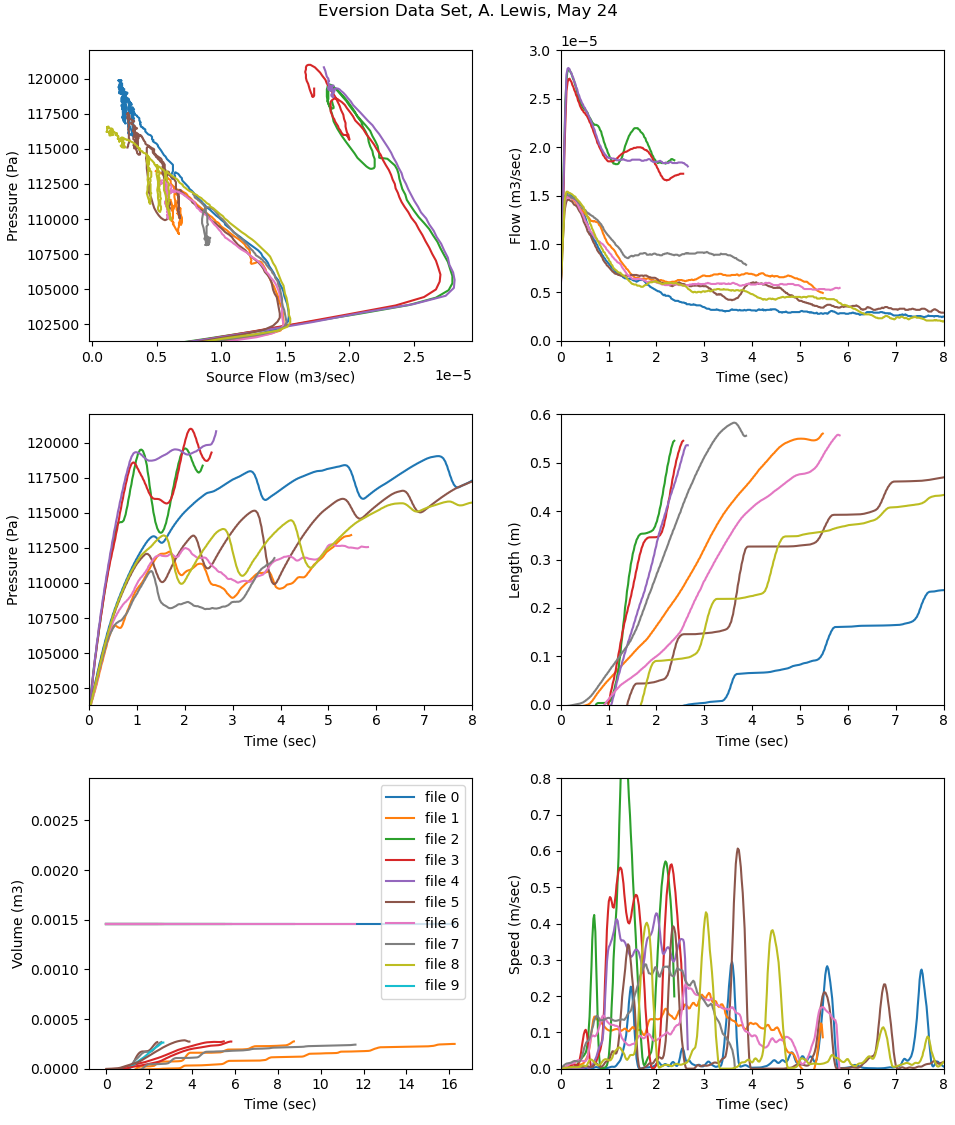
\includegraphics[width=.475\textwidth]{ExpDataExampleAll.png}
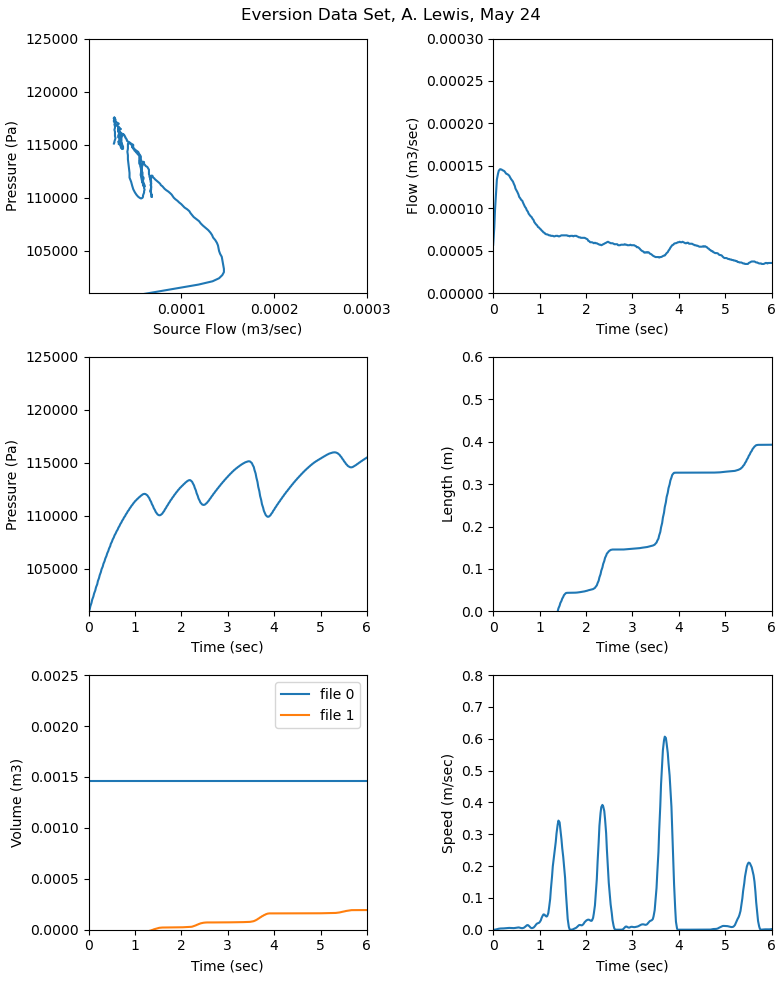
\includegraphics[width=.475\textwidth]{ExpDataExample.png}
\caption{Experimental data displaying dynamic characteristics of loaded eversion.  All data (Left), single example (Right) note different time axes for the two plots. (See Lewis, Fig 9. Loads: high inertia, high Friction)}
\label{Fig:experData}
\end{figure}

{\bf  ****    Resolve 10x flow rate hack!!!   *** }

Recently,  Lewis \cite{xxxx} measured some complex dynamic behaviors of a tube everting
inside
a straight support tube of approximately the same diameter (25mm)
as the inflated tubing material (Figure \ref{Fig:experData}, Left panel).
Data consist of 9 trials on 3 tubes.  Tube \#1 had 4 trials, tube \#2 had
2 trials, and tube \#3 had 3 trials.
% Andy: housing dims:   0.0013976 m^3. Accounting for the reel assembly, it's 0.00125562 cubic meters.
Tubes were supplied by a reel which was free to rotate inside the pressure vessel (housing).
Variable loads could be applied to the reel including  inertia and coulomb friction.
Applied loads are given in Table \ref{table:loadsAndTrials}.

There are two distinct clusters of responses, five slower and three faster (particularly clear
in the flow plots (top row). The three datasets having higher flow rates in the top row of Figure
\ref{Fig:experData} are the three trials of tube \#3.

One experiment which displays several interesting evertion characteristics
is shown in Figure \ref{Fig:experData}, Right Panel.
Referring first to the length-vs-time plot (middle right), we see a start-stop or staircase
behavior sometimes seen with eversion under relatively constant input pressure.   It
should be noted that the selected eversion experiment (Right panel) was loaded by ``high" inertia and
``High" friction applied to the reel.  Velocity (lower right) indicates a series of peaks where the eversion
``breaks-free" but then stops again a short time later giving length-vs-time a stair-step characteristic.

Pressure (middle left) first grows for about 1 second without corresponding eversion motion, and
then oscillates in approximate synchrony with the velocity peaks.

Finally, the pressure-flow phase plot (top left) shows a predominantly diagonal straight line slope.
Flow grows rapidly and then the trajectory proceeds from
lower right (high initial flow with low pressure) to upper left (lower flow, higher pressure).
The trajectory makes loops to lower pressures and back up to the slope at higher pressures.  These
loops correspond in time to the pressure oscillations (middle left).

These dynamic characteristics (start-stop bursting, pressure oscillations, diagonal phase trajectory, and
downward loops) were not all present under all experimental conditions.  In summary then, depending on
factors to be determined, some or all of these characteristics may or may not be present in a given
free eversion run.

\subsection{Simulation Goals}
The goals of this simulation are:
\begin{enumerate}
  \item Increase fundamental understanding of the eversion process.
  \item Identify key parameters capable of representing the complex dynamic characteristics above.
  \item Identify values and value ranges for unknown parameters which fit individual experiments.
  \item Clearly segregate the parameters into known, measured quantities vs. free parameters.
  \item Codify an efficient manual method for parameter identification.
\end{enumerate}

In any simulation study caution must be exercised when there are a large number of free parameters
as there may be several combinations of parameters or manifolds in the parameter space which
may fit any dataset.   In Section \ref{Sec:Params}, below, we review the overall parameter set and
classify the parameters into known, independently measureable parameters vs free parameters.


\subsection{Dynamic Model}
The dynamic model of an eversion drive system includes;
\begin{itemize}
  \item An everting tube of length $L$ and growth rate $\dot{L}$.
  \item A pressurized housing
  \item A reel with rotation $\theta, \dot{\theta}, \ddot{\theta}$, on which tubing is rolled having inertia (assume fixed) of
  $J$ and radius $r$.
  \item A brake which applies a Coulomb friction torque to the reel
  \[
    \tau_c = C\mathrm{sgn}(\dot{\theta})
  \]
  \item A ``crumple zone" in which eversion material can accumulate
  between the reel and the everting tube. The length of material in
  the crumple zone is $L_c >= 0$.
  \item Eversion happens when the eversion force (pressure $\times$ face area of the tube) exceeds any retarding forces.
  \item Forces which can oppose eversion include,
  \begin{itemize}
    \item drag forces and inertial forces required to pull the tubing material
    inside the deployed tube,
    \item reel inertia and reel friction resulting from unspooling material (only when $L_c = 0$).
  \end{itemize}
\end{itemize}

\noindent
The everting tube can be in one of two states:
\begin{itemize}
  \item GROWING (the tube is actively everting, $\dot{L}>0$)
  \item STUCK (the tube is not growing due to insufficient everting force, $\dot{L}=0$)
\end{itemize}
and the reel/crumple zone can be in one of two additional states:

\begin{itemize}
  \item TAUGHT (the crumple zone has zero length , $L_c = 0 $)
  \item SLACK (there is material in the crumple zone, $L_c > 0$)
\end{itemize}

Together the system can be in four states comprising the permutations
of these two state variables.

\section{Model Structure and System Equations:}

We will consider two possible structures:

A {\it one-compartment} model (Figure \ref{Fig:TwoStructures}, Left)
assumes that first-order pressure dynamics are present between a source of   pressure  ($P_{source}$ from a compressor, regulator, or tank accumulator)
and a single  everting tube system volume (housing plus tube volume, $V_{et} = L\times \pi r^2$.) with uniform pressure, $P$.

The {\it two-compartment} model(Figure \ref{Fig:TwoStructures}, Right)
assumes that additional first-order pressure dynamics are present between
the housing volume (pressure, $P_1$, volume $V_{housing}$ and the tube system volume ($V_{et}$ as above).

For both structures, we can make the tube radius a function of its length, $R_{et}(L)$.   This can simulate novel designs with varying
radii exploiting new ET
fabrication methods such as laser welding or CNC heat sealing.

\begin{figure}[h]\centering
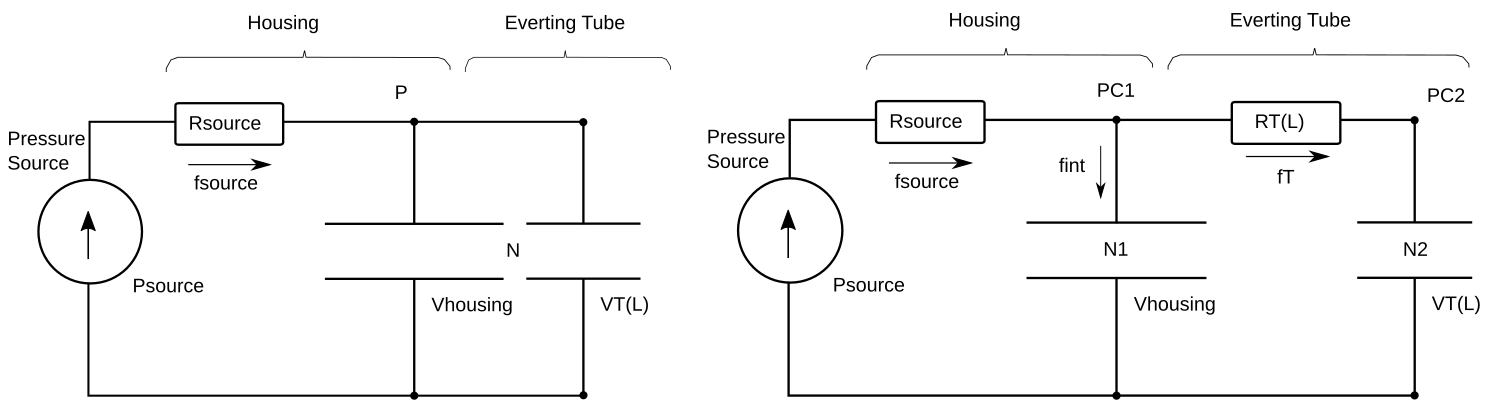
\includegraphics[width=0.9\textwidth]{Fig_OneAndTwoCompartment.png}
% 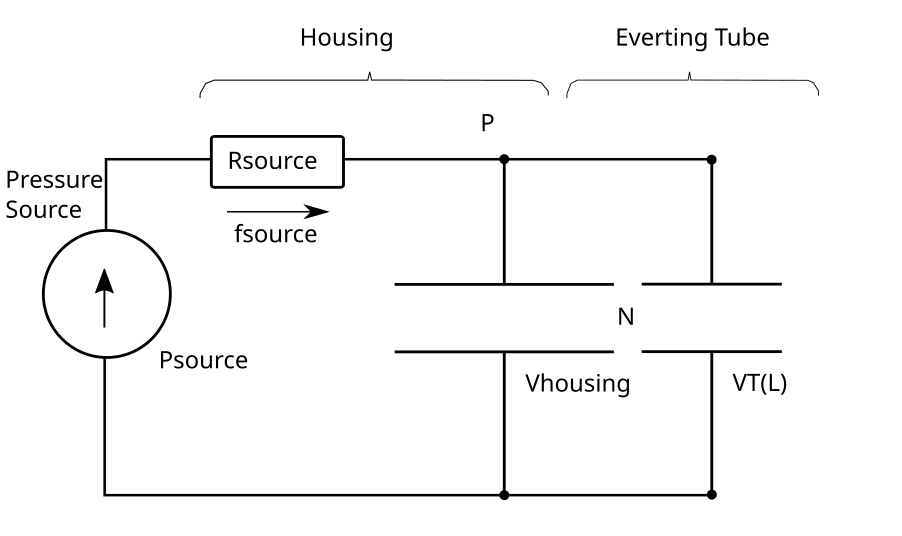
\includegraphics[width=.475\textwidth]{Figure_OneCompartment.png}
% 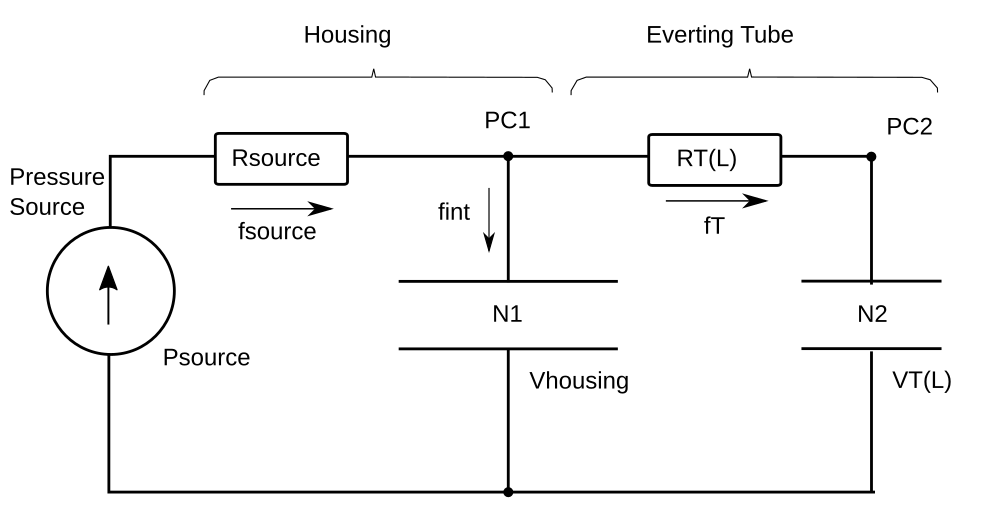
\includegraphics[width=.475\textwidth]{Figure_TwoCompartment.png}
% 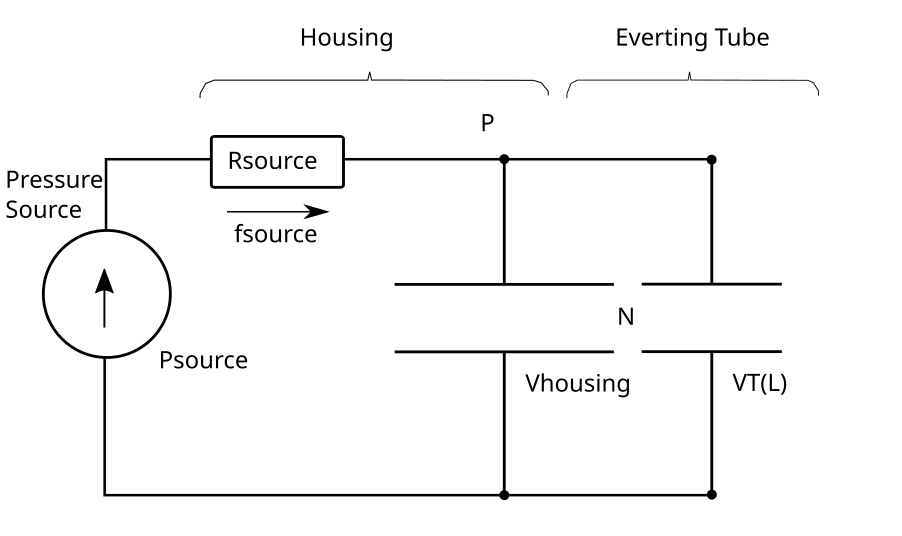
\includegraphics[height=1.5in]{Figure_OneCompartment.png}
% 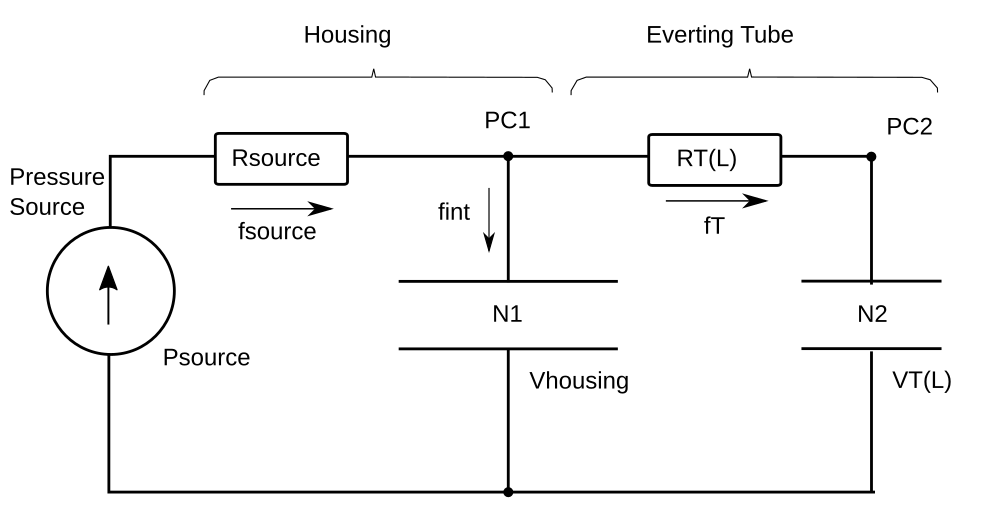
\includegraphics[height=1.5in]{Figure_TwoCompartment.png}
\caption{Two model structures applied to eversion experiments of
Fig. \ref{Fig:experData} expressed as simple electric circuits.
One compartment model (Left) lumps the
housing volume and tube volume together. Two compartment model (Right)
introduces length-dependent resistance between the housing and tube, $RT(L)$, to split the pressure state, $P$ into two states, $P_{C1}, P_{C2}$.}\label{Fig:TwoStructures}
\end{figure}


After setting initial conditions (see below), we model eversion dynamics by:
\begin{enumerate}
  \item Computing volume and pressure.
  \item Computing forces applied to the eversion tip and accounting for the mechanical advantage (everting material speed is $2\times\dot{L}$, Pressure applied to everting front develops 1/2 the everting force expected from $P\times A$.)

  \item Selecting the dynamic mode from the four combined states above and computing accelerations.
  GROWING or STUCK state is selected by pressure thresholds (related to net
  eversion force by $F=PA(L)$.
  TAUGHT or SLACK state is selected by checking length of
  the crumple zone material. Then, according to the dynamic mode, summing forces, equating to  zero, solving for tube and reel accelerations.

  \item Eversion does not come to an instant halt. We  empirically model a short exponential decay of velocity as tube decelerates.

  \item Implement the transitions between states STUCK, Growing, and TAUGHT,  SLACK. %item5


  \item  Integrate acceleration and velocity to update state variables.  %item6


\end{enumerate}

\noindent
Specifically for the one-compartment model:

\begin{enumerate}
\item
\begin{equation}\label{eqOneCompartmentVol}
V_t = V_{housing} - V_{contents} + L  A
\end{equation}
$V_t$ includes both the reel housing volume (minus the volume of its contents)
and the everted tube volume $Vet(L)$ with cross sectional area $A(L)$
where
\beq
A(L) = \pi Ret(L)^2
\eeq
where $Ret(L)$ is initially a constant radius, but can also
be a function describing a diameter profile manufactured into the
everting tube. Alternatively, $Ret(L)$ can describe a constraining
tube of radius $R_C(L)$ such that
\beq
R_C(L) <= Ret(L)
\eeq
When the radius is not constant, tube volume is computed by

\beq
Vet = \pi \int_0^L Ret(L)^2 dL
\eeq

From the ideal gas equation:
\begin{equation}\label{eqOneCompartmentPress}
P = \frac{N  RT}{ V_t}
\end{equation}

where $N$ is the molar mass of gas in the system, $R$ is the gas constant, and $T$ is the temperature
in $^\circ$K.  We assume temperature is constant during eversion (isothermal boundary condition).
%
% \begin{figure}\centering
% 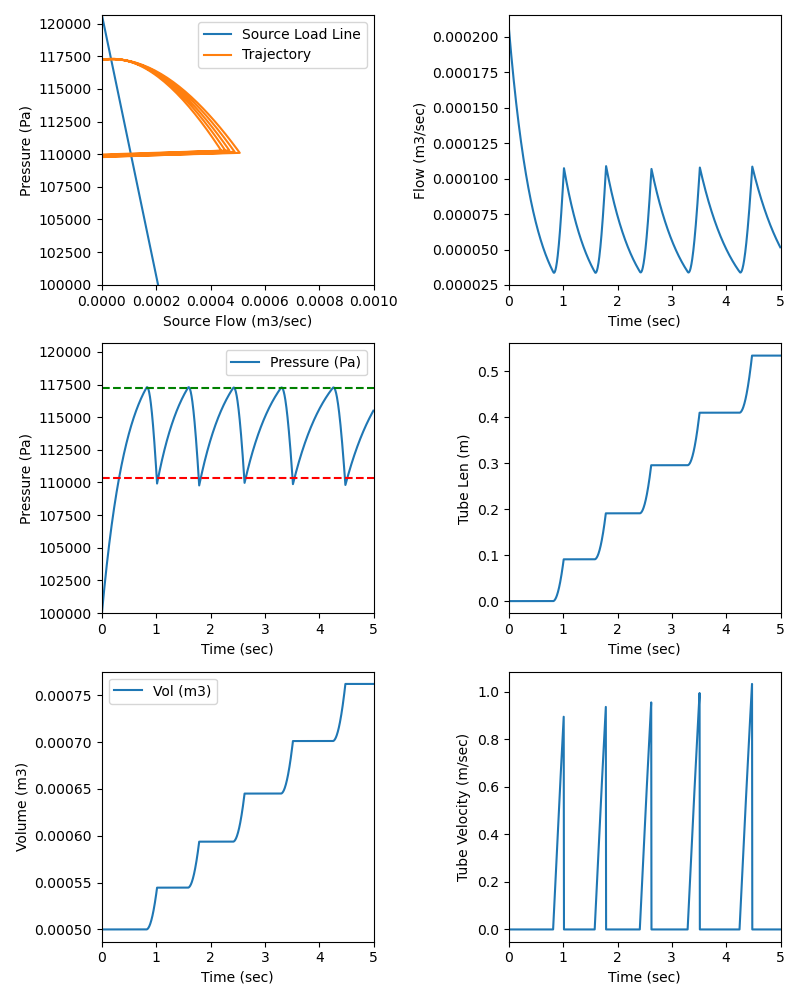
\includegraphics[width=.75\textwidth]{Figure_9HhiI_hiTf_baseline.png}
% \caption{Simulation Run with approximate qualitative match.  (See Lewis, Fig 9, hiI, hiTf)}
% \label{Fig:baselineResults}
% \end{figure}


\item

Computing Forces:


\begin{equation}
  F_{ever} = \mathrm{max}(0, PA/2)
\end{equation}
\beq
  F_{c} = \tau_{Coulomb} / r
\eeq

Coulomb friction is independent of velocity so does not get scaled by the
$2\times$ mechanical advantage.

\item Computing acceleration according to the four dynamic states:

GROWING and SLACK:

\beq
\ddot{L} = \frac{F_{ever} - F_D(FL,\dot{L})-F_C}  {M_T/2}
\eeq

\beq
\ddot{\theta} = - \tau_{Coulomb}/J
\eeq
where $M_T$ is the mass of inside tubing, pulled at $1/2$ speed
by the eversion process, and $J$ is the rotational inertia of
the tubing reel inside the housing. We assume $J$ is constant
(despite some material being unspooled) and that
$\tau_{Coulomb}$ is a known constant torque. Finally tubing mass is proportional to length:
$M_T = L \cdot \mathrm{ET\_mass\_per\_mm} $.

GROWING and TAUGHT:

%         Lddot = (1/Mt + (rReel\_SIu**2/J) ) * ( F_ever - Fdrag(L,Ldot) - Fcoulomb )
%         th_ddot = Lddot/rReel\_SIu
\beq
\ddot{L} =(F_{ever} - F_D - F_C) /  (M_T/2 + J/r^2)
\eeq

\beq
\ddot{\theta} = \ddot{L}/r
\eeq
\noindent
in this state reel acceleration is kinematically linked to tube growth.

STUCK and (SLACK or TAUGHT):


%         alpha = 2000 * dt  # empirical fit
%         Lddot = -1 * max(0, alpha * Ldot)
%         th_ddot = tau_coulomb/J



\beq
\ddot{L} = -1 * \mathrm{dmax}(0, \alpha * \dot{L})
\eeq

\beq
\ddot{\theta} = - \tau_{Coulomb} / J
\eeq
where $\alpha$ is an empirical time constant modeling the dynamics of eversion stopping.

Modeling flow from the pressure source (Thevenin equivalent):
\begin{equation}\label{eqOneCompartmentflow}
Fl_{source} = \frac {P_{source}-P} {R_{source}}
\end{equation}

Converting airflow ($m^3/sec$) to rate of molar mass flow:
\begin{equation}\label{eqOneCompartmentNdot}
\dot{N} = Fl_{source} \cdot \mathrm{moles\_per\_m3}
\end{equation}

Model velocity and length dependent eversion force which is resistance to pulling out eversion material:
%     everDrag =   2 * (pd['Kdrag'] +  pd['K2drag'] * L) * Ldot

\begin{equation}
F_D(L,\dot{L}) = \mathrm{max} \left( 2  (  K_{D} + L  K_{2D} ) \dot{L} , F_{end} (L)  \right )
\end{equation}

Where the factor of two accounts for everting material going at twice tube growth rate, $\dot{L}$,
and $F_{end}$ is a function to model the everting tube material running into its hard stop:
% Fsteadystate = pd['Psource_SIu']*np.pi*et.Ret(L,pd)**2
% F_limit = (L/pd['Lmax'])**7 * Fsteadystate
\beq
F_{end}(L) = (L / Lmax)^7  P_{source} \pi Ret(L)^2
\eeq
Update length of  crumpled material (if any)
\beq
L_C = \mathrm{max}(0,  r\theta - L)
\eeq




\item Implement state transitions

We have a switching model to replicate observed intermittent starting and stopping of eversion
which updates the state based on current pressure:
\begin{equation}
    \mathtt{state} =
    \begin{cases}
      \mathrm{GROWING}, &  P > P2 \\
      \mathrm{unchanged}, & P1 <= P <= P2 \\
      \mathrm{STUCK},   &  P < P1
    \end{cases}
\end{equation}

%
%
% We are currently investigating changing this switching model to one based on thresholding
% net eversion force rather than tip surface pressure:
% \begin{equation}
%     \mathtt{state1} =
%     \begin{cases}
%       \mathrm{GROWING},   &  F_{ever} > F2 \\
%       \mathrm{unchanged}, &  F1 <= F_{ever} <= F2 \\
%       \mathrm{STUCK},     &  F_{ever} < F1
%     \end{cases}
% \end{equation}


We update the crumple state depending on the length of the crumple
zone ($L_C$) as
\begin{equation}
    \mathtt{state2} =
    \begin{cases}
      \mathrm{TAUGHT},  &  L_C <=0 \\
      \mathrm{SLACK},   &  L_C  > 0
    \end{cases}
\end{equation}

\item Integrate state variables.

Finally, we integrate the state variables:
\begin{equation}
\begin{aligned}
  \dot{L} &= \dot{L} +  \ddot{L}  dt \\
  L       &= L + \dot{L}  dt \\
  \dot{\theta} &= \dot{\theta} + \ddot{\theta}dt \\
  \theta &= \theta + \dot{\theta} dt\\
  N &= N + \dot{N}  dt\\
\end{aligned}
\end{equation}
\noindent
and, if necessary ($Ret(L)$ is not constant),
\beq
Vet = Vet +  \pi Ret(L)^2  \; \dot(L)
\eeq

\end{enumerate}


\subsection{Initial Conditions}
For a typical simulation, the initial conditions are
\begin{equation}
\begin{aligned}
  P &= 1 \; \mathrm{atmosphere}\\
  {\tt state1} &= STUCK \\
  {\tt state2} &= TAUGHT \\
  N &= N(V_{housing} - V_{contents}) / RT \\
  L &= 0\\
  \dot{L} &= 0\\
  \ddot{L} &= 0\\
\end{aligned}
\end{equation}

\subsection{Parameters}\label{Sec:Params}
The model parameters are classified in Table \ref{Tab:paramClass}.
The first 10 parameters are independently measured or otherwise known.  For example,
atmospheric pressure (Patmosphere) and room temperature (T) are known or
measured constants.
Reel parameters rReel, J, Tau\_coulomb, and Vhousing\_m3 are known from CAD files
and independently confirmed by measurements\cite{Lewis2024XX}.
Inertia, J, and coulomb friction were set to three different levels during
experimentation, ``low", "medium," and "high" as indicated in Table \ref{Tab:paramClass}.
The maximum tubing length, Lmax, is known at fabrication time (about 0.6m).
Sometimes it was modified within a narrow range  by matching the end length
between experiment and simulations.

\begin{table}
\begin{tabular}{l|l|l|l|p{1.35in}|l}
Parameter     &  Class     & Value   & Units     & Description      & source \\ \hline
ET\_radius     &  Known     & 12.5    &  $mm$       & Tube radius      & tube design \\
%     J = 1.0E-4*[ 4.67, 5.10, 5.64][Ji]
J             &  Known     & [ 4.67, 5.1, 5.64]$\times10^{-4}$ &  $kg/m^2$    & Reel inertia     [Lo, Med, Hi]& design, tests \cite{Lewis2024XX} \\
Tau\_coulomb    &  Known     &[ 2.9, 17.4, 69.4]$\times10^{-3}$&  $Nm$       & Coulomb friction torque on reel [Lo, Med, Hi]  & design, tests \cite{Lewis2024XX} \\
Lmax          &  Known     & 0.5-0.8 &  $m$        & Tube length      & tube design  \\
Patmosphere   &  Known     & 101.325 &  $kPa$      & Atmospheric pressure & \\
RT            &  Known     & 2.5E+3 &   $m^3 Pa/mol$   & Gas constant x temperature & Ref. \\
T             &  Known     & 2.95E+2 &  $^\circ K$    & Room temperature   & Thermometer \\
Vhousing\_m3   &  Known     &  1.256E-3 &  $m^3$      & Housing air volume  & CAD model \\
et\_MPM        &  Known     &  0.1    &  $kg$       & Tubing mass per meter  & measured \\
rReel         &  Known     &         &   $m$       & Reel radius & CAD model \\ \hline
ET\_Res\_ratio  &  Free      & 0.3---0.6 &  dimensionless &  ET resistance scale & manual tuning \\
K2drag        &  Free      & 0.16---4.0  &  $Nm$       & Empirical Fit    & manual tuning \\
Kdrag         &  Free      & 0.15---6.0   &  $N/m^2/sec$ & Empirical Fit & manual tuning \\
PBA\_static    &  Free      & 107---118.5  &  $kPa$      & Break-away pressure  & manual tuning \\
PHalt\_dyn     &  Free      & 61---116     &  $kPa$      & Eversion stopping pressure  & manual tuning \\
Psource\_SIu   &  Free      & 118---145    &  $kPa$      & Gas source pressure & manual tuning\\
Rsource\_SIu   &  Free      & (8---14)$\times10^7$ &  $Pa/m^3/sec$    & Slope of P-Fl load-line & manual tuning\\
Thresh. Taper & Free     &  640---3800  &  $Pa/m$      & Change in thresholds w/ length   & manual tuning\\
% Observation         & Param       & Orig. value   &  Modified Value  \\\hline
% Velocities too high  & ${\tt Kdrag}$  &   0.3     & 0.6          \\\hline
% Pressure thresholds converge with time& {\tt PBA\_static} & $1.17\times10^5 $Pa & $1.17\times10^5 - 500L$ Pa          \\\hline
% Pressure thresholds converge with time & {\tt PHalt\_dyn} & $1.17\times10^5 $Pa & $1.013\times10^5 + 500L$ Pa       \\\hline
% Pressure rise too slow  & $V_{housing}$   &  $0.5\times10^{-3}$ m$^3$   & $0.05\times10^{-3} $ m$^3$   \\\hline
% Peak Velocity too high  & $J$             &  $5.10\times10^4$  kg/m$^2$     & 10.2$\times10^4$  kg/m$^2$ \\\hline
\end{tabular}
\caption{Parameters used and their sources and values. }\label{Tab:paramClass}
\end{table}
% \vspace{0.175in}
%
% The modified parameter set is given in Section \ref{modParams} below.  Asterisks (*) denote iteratively changed parameters.
%
% Simulation with the modified parameters (Figure \ref{Fig:ModifParResults}) improve the model fit to data by
%     1) Shrinking loops on the pressure flow plot (upper left) are similar
%   to shrinking loops in experimental pressure-velocity plot'
%     2) Convergence of the eversion thresholds (center left) causes the shrinking loops above,
%     3) Peak velocities better match peaks of fig. 9, and match the pattern of the highest velocity
%   appearing near the center of travel.
%     4) With the modified parmeters there are about 2 bursts per second, similar to the experimental rate.


\section{Parameter Estimation from Data}

We used the following process  to fit parameters to an eversion data
record where the record consists of the following data as a function of time:

\begin{itemize}
    \item Pressure in the tube storage chamber ($Pa$)
    \item Air flow from source into tube storage chamber ($m^3/sec$)
    \item Length of the everted tube ($m$)
    \item Velocity of eversion (derived) ($m/sec$)
\end{itemize}


% These can be plotted multiple ways such as in Fig \ref{Fig:baselineResults} for example.

Simuation outputs can be plotted over the data to facilitate comparison.

We can then use the following procedure to iteratively tune  the free model  parameters to match a
particular experimental run.
% Other parameters such as the tube reel radius, inertia, and braking
% friction are readily measured independently \cite{Andy Papers}  and not fit to the eversion experiments.

\begin{enumerate}
    \item  Adjust load line pressure intercept.

    {\bf Data Focus: } Pressure/Flow curves (upper left):\\
    {\bf Procedure: } Adjust Psource\_SIu to move the load line and sim trajectory (they should overlap)
    up and down.  Adjust Rsource\_SIu to adjust its slope (higher values slope down more).

    \item Adjust stop-start thresholds.

     {\bf Data Focus: } Pressure-Time curves (middle left):\\
    {\bf Procedure: } Adjust PBA\_static up or down to match the pressure peaks in experiment (green dashed).
    Adjust PHalt\_dyn  up or down to match the pressure valleys.

    \item Adjust threshold taper.

     {\bf Data Focus: } Pressure-Time curves (middle left):\\
    {\bf Procedure: } Adjust Threshold Taper up or down to speed or slow down convergence of the thresholds.

    \item Adjust Friction or drag

     {\bf Data Focus: } Length-Time curves (middle right):\\
    {\bf Procedure: } Adjust the viscus drag constant of tubing (K\_drag) up or down to match the overall slope
    of the data trace.
    Adjust max tubing length (Lmax) to match stopping point of data.

    \item Experiment with other parameters or go back and repeat the procedure.

\end{enumerate}




%
%   17-Jul: New simulation while going back to one-compartment
%
%    Compared "initialParameters" and tuned them for dataset 6:
%                             hi-inertia, hi_fric, tube-2 trial22
%

\begin{figure}\centering
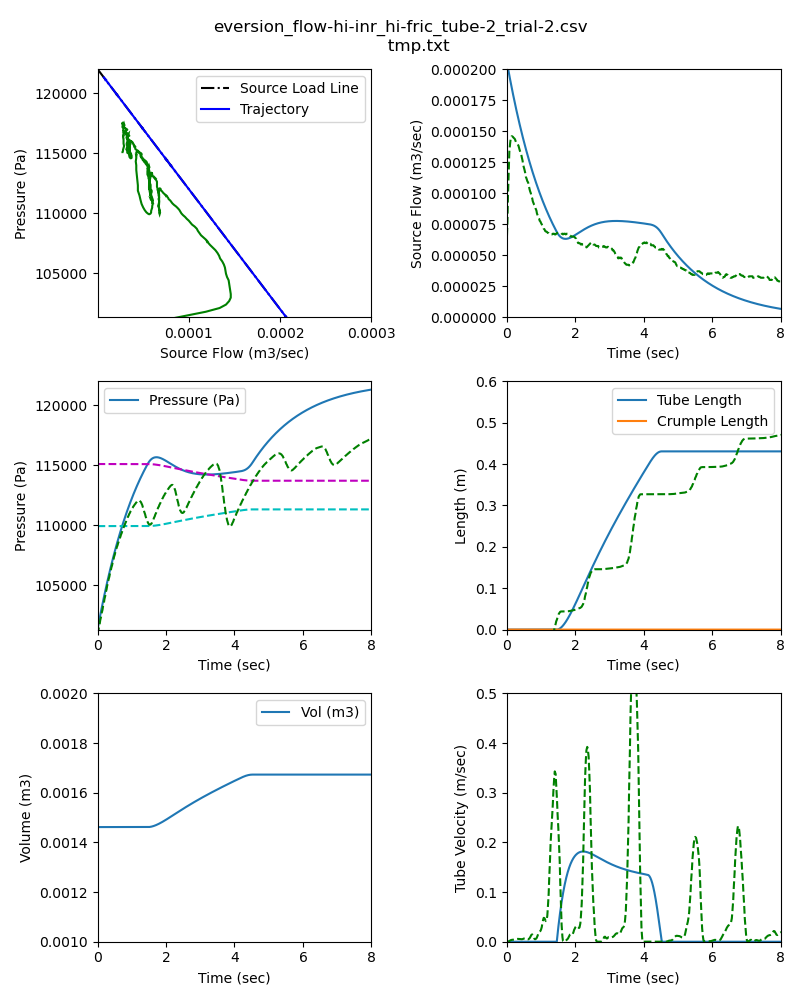
\includegraphics[width=.75\textwidth]{Set6wInitialParams.png}
\caption{Comparison of one experimental run (green dashed line)
with a simulation (solid blue line)
using an initial set of parameter values (Table \ref{Tab:InitialParams}).}
\label{Fig:InitialSimCompare}
\end{figure}


We modeled one experiment (hi inertia, hi friction, tube-2, trial-2)
simulating the model with
an initial set of parameters (Table \ref{Tab:InitialParams}).

A number of features in the experimental data are absent from the simulation
output
including: load line between pressure and flow are misaligned by an offset and
a slight slope difference (Figure \ref{Fig:InitialSimCompare}, upper left),
Pressure changes smoothly over time in the simulation without oscillations
evident in the experimental data (middle left), and tube length grows smoothly
in the simulation compared with discontinuous growth in the data (middle right,
lower right).

Using the above procedure, we made the following changes to improve match
between simulation and experiment:

\begin{enumerate}
    \item Reduce source pressure to match the load line to the predominant Pressure-Flow slope.
    \item  Adjust pressure thresholds for ``Break-Away" and ``Halting" and
    drag coefficients to match the
    bursty motion of the experimental data.
    \item  Adjust source pressure, drag parameters, and threshold taper to
    increase matching.
\end{enumerate}


\begin{figure}\centering
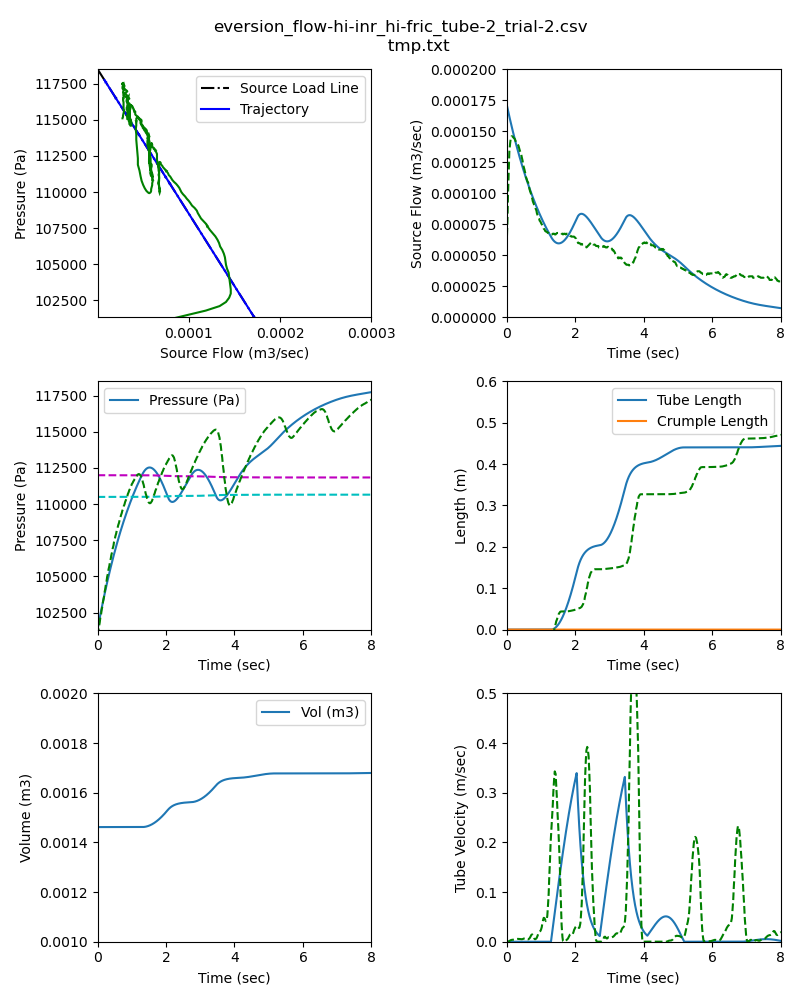
\includegraphics[width=.75\textwidth]{Set6wFinalParms.png}
\caption{The same simulation and data (See Lewis, Fig 9, hiI, hiTf) with manually tuned parameter values (Table \ref{Tab:FinalParams}}
\label{Fig:FinalSimCompare}
\end{figure}

\begin{table}[h]
\centering
\begin{tabular}{l|l|l}
Parameter     &  Value   & Units \\ \hline
ET\_RofL\_mode  &  constant & text \\
ET\_radius  &  1.2500E-02 & m \\
J  &  5.6400E-04 & kg/m2 \\
K2drag  &  1.0000E+01 & Nm \\
Kdrag  &  8.0000E+00 & N/m2/sec \\
LLine\_SIu  &  1.0000E-08 & m3/sec/Pascal \\
Lmax  &  6.0000E-01 & m \\
PBA\_static  &  1.1511E+05 & Pascals \\
PHalt\_dyn  &  1.0994E+05 & Pascals \\
Patmosphere  &  1.0132E+05 & Pascals \\
Psource\_SIu  &  1.2201E+05 & Pascals \\
RT  &  2.4560E+03 & ?? \\
Rsource\_SIu  &  1.0000E+08 & Pa/m3/sec \\
T  &  2.9540E+02 & K \\
Tau\_coulomb  &  6.9400E-02 & Nm \\
Threshold  Taper & 3.2319E+03 & Pa/m \\
Vhousing\_m3  &  1.4616E-03 & m3 \\
dt  &  2.5000E-03 & sec \\
et\_MPM  &  1.0000E-01 & kg/m \\
rReel  &  1.0900E-02 & m \\
% th\_dot\_minCoulomb   &  5.0000E-02  & rad/sec\\
\end{tabular}
\caption{Initial parameter values for the simulation before parameter tuning (Figure
\ref{Fig:InitialSimCompare}}\label{Tab:InitialParams}
\end{table}


After modifications to some parameters (Table \ref{Tab:FinalParams}),
the simulation shows better match to the pressure-flow load line, pressure
oscillations during growth, and bursty length changes during growth.

Some remaining differences include: slower rate of change of pressure
with time after the initial pressure rise (during eversion) and
lack of looping cycles visible in the upper left of the pressure-flow
plot.  Indeed from the one-compartment model structure (Figure \ref{Fig_OneAndTwoCompartment}) it is clear that the simulation is
constrained to the diagonal load line.

\begin{table}\centering
\begin{tabular}{l|l|l}
Parameter    &     Value    &   Units \\ \hline
ET\_RofL\_mode  &  constant & text \\
ET\_radius  &  1.2500E-02 & m \\
J  &  5.6400E-04 & kg/m2 \\
K2drag*  &  5.0000E-01 & Nm \\
Kdrag*  &  1.0000E+00 & N/m2/sec \\
LLine\_SIu  &  1.0000E-08 & m3/sec/Pascal \\
Lmax*  &  6.5000E-01 & m \\
PBA\_static*  &  1.1200E+05 & Pascals \\
PHalt\_dyn*  &  1.1050E+05 & Pascals \\
Patmosphere  &  1.0132E+05 & Pascals \\
Psource\_SIu*  &  1.1850E+05 & Pascals \\
RT  &  2.4560E+03 & ?? \\
Rsource\_SIu  &  1.0000E+08 & Pa/m3/sec \\
T  &  2.9540E+02 & K \\
Tau\_coulomb  &  6.9400E-02 & Nm \\
Threshold Taper* & 3.5000E+02  &  Pa/m \\
Vhousing\_m3  &  1.4616E-03 & m3 \\
dF1dL  &  3.6364E+00 & N/m?? \\
dt  &  2.5000E-03 & sec \\
et\_MPM  &  1.0000E-01 & kg/m \\
rReel  &  1.0900E-02 & m \\
\end{tabular}
\caption{Final  parameter values after parameter tuning on the
same data set (Figure \ref{Fig:FinalSimCompare}). '*' indicates parameter was
modified to improve fit.}\label{Tab:FinalParams}
\end{table}

\clearpage


\section{Model Refinements}


\subsection{Multiple compartment model}
% So far, pressure and flow dynamics have considered the tubing supply chamber and the everted tubing to be a single compartment
% for computation of volume (Eqn \ref{eqOneCompartmentVol}) and pressure (Eqn \ref{eqOneCompartmentPress}) yielding a single
% flow (Eqn \ref{eqOneCompartmentflow}).

The results of the one-compartment model illustrate a limitation that its
pressure-flow behavior is limited to a straight line.
% We introduced a two-compartment
% model to account for airflow dynamics in supplying flow to the tube from the
% housing as it
% everts and possible differences between the tube-tip pressure and the housing
% pressure.
We noted loops in the pressure-flow plane (Figure \ref{Fig:FinalSimCompare},
upper-left)
in which a growing ET deviated
significantly from the source load line.   This indicates that air pressure does not instantaneously equilibrate
along the ET, but instead takes time to flow from the tubing compartment down to new volume at the growing tip.
A lumped parameter model of this flow can be formed of two compartments: one
compartment is the reel housing from
which the tube is everted, and the second compartment is
the tubing.   A flow resistance, $R_T(L)$, connects the two chambers and this resistance increases with length.  Initially we assume that the
flow resistance between compartments is a fixed ratio (ET\_Res\_ratio) of the
source resistance (Rsource\_SIu).  Length dependence of the resistance will
be introduced later if needed.
The tubing volume increases with length (as it did in Eqn \ref{eqOneCompartmentVol}).
Such a model is shown in Figure \ref{Fig:OneAndTwodTwoCompartment} (Right).
% Such a model is shown in Figure \ref{Fig:TwoCompartment}.
%
% \begin{figure}[h]\centering
% % 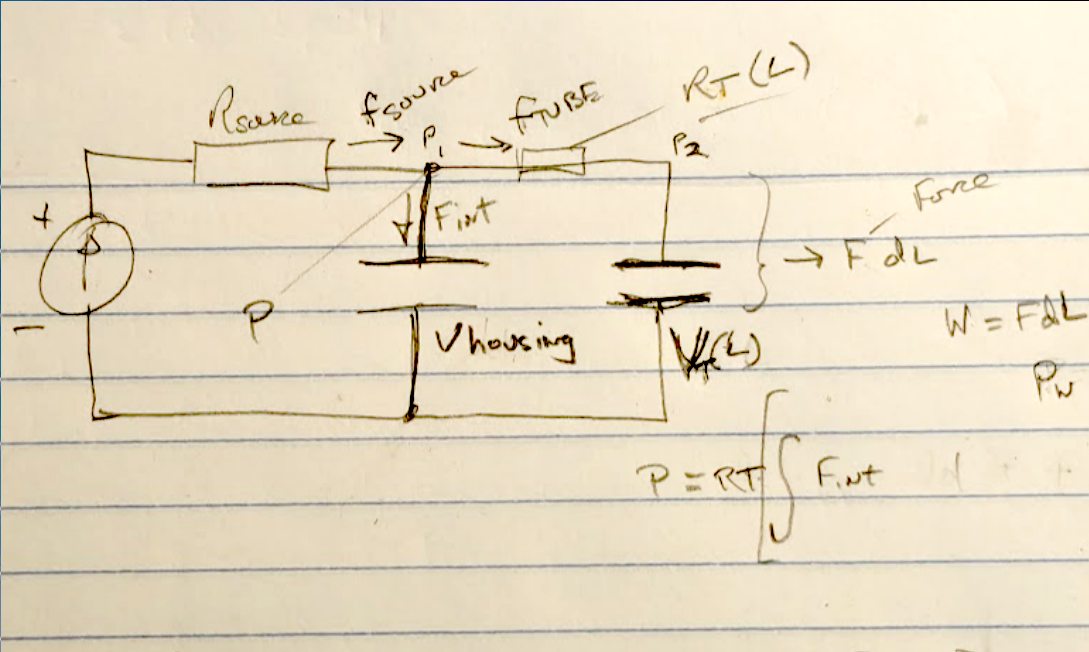
\includegraphics[width=.5\textwidth]{Photo_TwoCompartment.png}
% 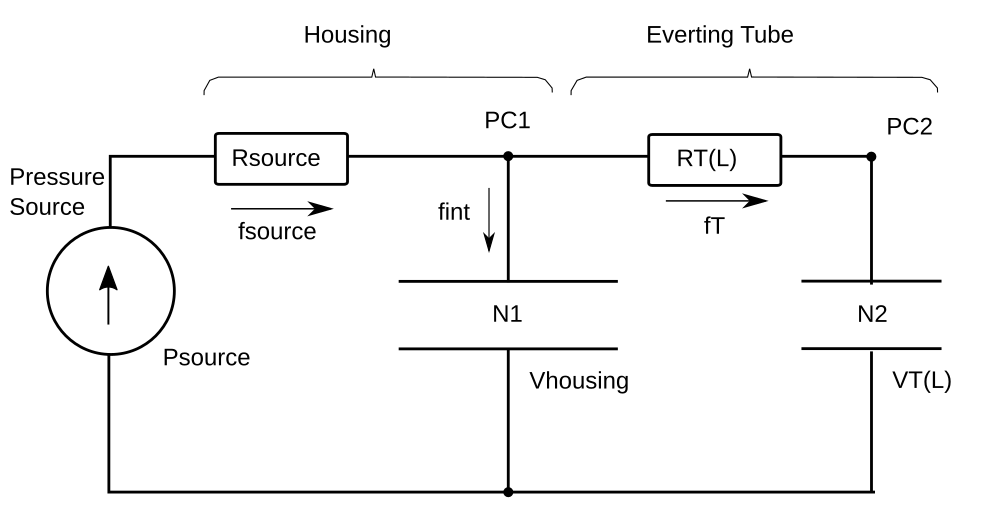
\includegraphics[width=.5\textwidth]{Figure_TwoCompartment.png}
% \caption{Two compartment, lumped parameter model. }
% \label{Fig:TwoCompartment}
% \end{figure}

Two add the second compartment, representing the everting tube volume and associated
flow, we need to expand our model state variables as follows:

\beq
\begin{aligned}
N, \dot{N}     &\to \{ N_1, N_2, \dot{N}_1, \dot{N}_2\}\\
V_{t}          &\to \{V_{housing}, V_T(L)\}\\
f_{source}     &\to \{f_{source}, f_{int}, f_{T} \}  \\
P              &\to \{ P_{C1}, P_{C2} \}
\end{aligned}
\eeq where
$N_1$ and $N_2$ are the molar quantity of air in the housing and tube respectively,
$f_i$ are the respective flows indicated in Figure \ref{Fig:OneAndTwoCompartment}
(Right), and
$P_{C1}$ and $P_{C2}$ are the pressures in the housing and tube respectively.



We then have new equations to replace or expand Equations \ref{eqOneCompartmentPress}, \ref{eqOneCompartmentflow}, and \ref{eqOneCompartmentNdot}
as follows:

\beq
\dot{N_1} = ( f_{source}-f_{int}-f_T ) \cdot \mathrm{moles\_per\_m3}
\eeq

\beq
\dot{N_2} =   f_T \cdot \mathrm{moles\_per\_m3}
\eeq

\beq
P_{C1} = \frac {N_1RT}  {V_{housing}}
\eeq

\beq
P_{C2} = \frac {N_2RT}  {V_T(L)}
\eeq

\beq
f_{source} = (P_{source}-P_{C1}) /  R_{source}
\eeq

\beq
f_{T} = (P_{C1}-P_{C2}) /  R_{T}(L)
\eeq

\beq
f_{int} = f_{source} - f_T
\eeq

\section{Results of Two Compartment Model}

\begin{figure}[h]\centering
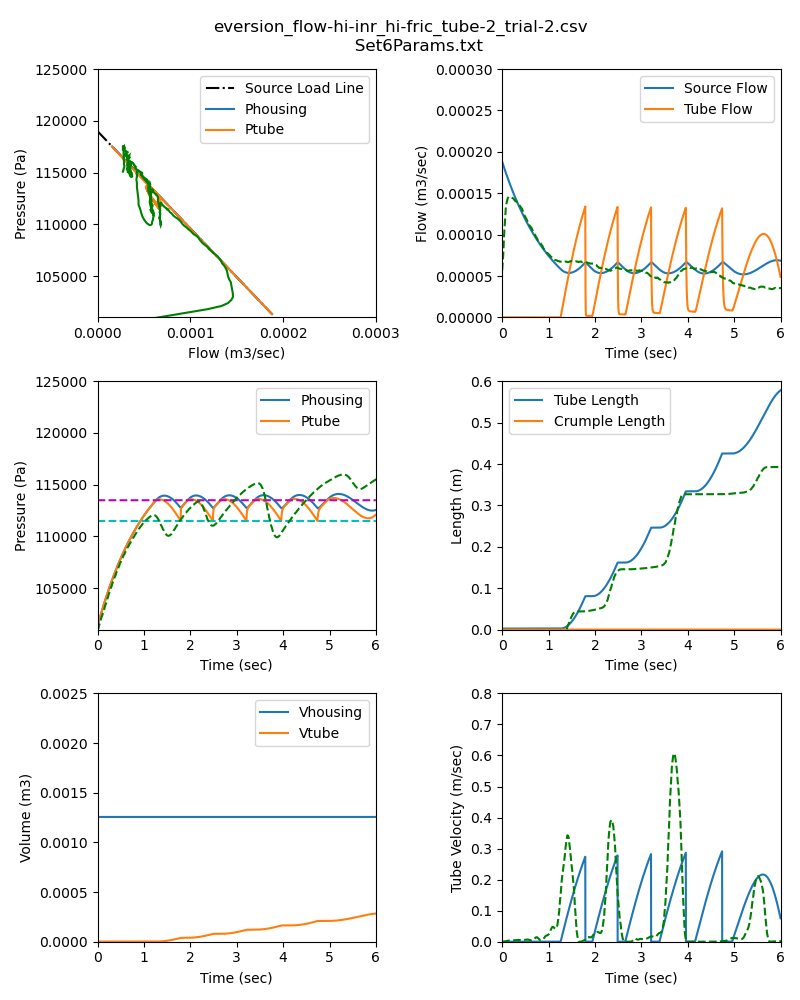
\includegraphics[width=.75\textwidth]{2CompSimulationSet6.png}
\caption{Two compartment model compared with same data as Figure \ref{}.
Two compartment model allows simulation to deviate from the diagonal load line (orange trace,
Upper Left).}
\label{Fig:2CompS6}
\end{figure}


The same data set as in Figure \ref{Fig:FinalSimCompare} were simulated with the two-compartment version of the model (Figure \ref{Fig:2CompS6}).
% Volume of the ET was a function of length, $L$.
Flow resistance between reel housing (compartment 1) and
the ET was approximated by a ratio of Rsource\_SIu.
Parameter set is given in Table \ref{Tab:TwoCompFitParams}.


\begin{table}\centering
\begin{tabular}{l|l|l}
\end{tabular}
\caption{Parameter values for the two-compartment model fit (Figure \ref{Fig:TwoCompSimCompare}).
}\label{Tab:FinalParams}
\end{table}



Results from Tube 1, Trial 2 (hi inertia, hi friction) are given in Figure \ref{Fig:2CompS6}.
Notably, the simulated tube pressure deviates below the source loadline during the start-stop
oscillations similar to the experimental data.

\clearpage


\subsection{Additional Two-Compartment Fits}

\begin{figure}[h]\centering
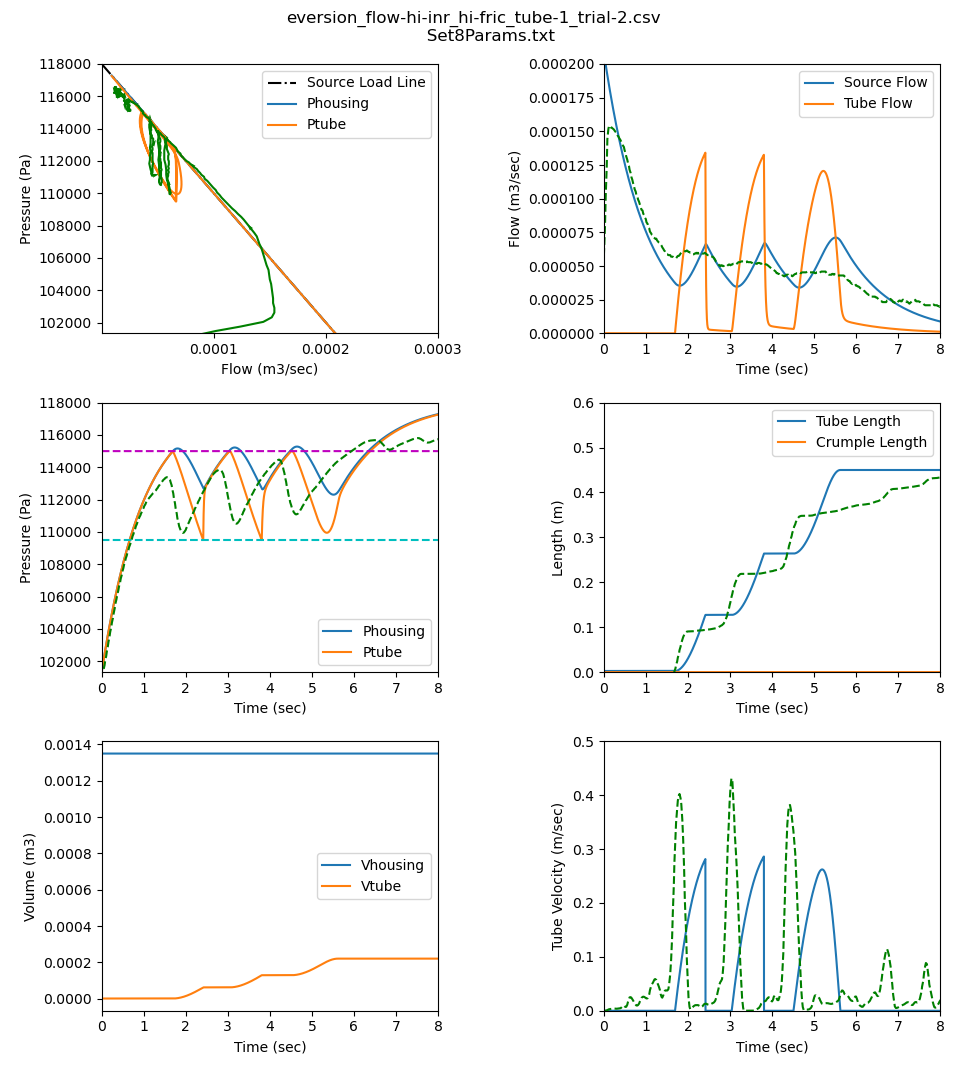
\includegraphics[width=.75\textwidth]{2CompSimulationSet8.png}
\caption{Two compartment model compared with simulation (See Lewis, Fig 9, hiI, hiTf)}
\label{Fig:2CompS8}
\end{figure}


\subsection{Varying tube profile}

While most ET research uses tubing of constant diameter, the effective diameter of an ET can vary with
length in two main ways.   First, the tube can be fabricated with variable diameter by thermal welding of two sheets.
Second, tubing of constant diameter may be everted into a tubular space of changing diameters.
While the mechanics of eversion will in general be different in these two cases, we will initially ignore that difference
and make tube diameter a function of eversion distance $L$, $V(L)$.

Tube profiles

Simulations





%  Use name of bibliography files without .bib extension
\bibliography{flowMOdel}
\end{document}
